%----------------------------------------------------------------------------------------
%	PACKAGES AND OTHER DOCUMENT CONFIGURATIONS
%----------------------------------------------------------------------------------------

\documentclass[
11pt, % Main document font size
a4paper, % Paper type, use 'letterpaper' for US Letter paper
oneside, % One page layout (no page indentation)
headinclude,footinclude, % Extra spacing for the header and footer
BCOR5mm, % Binding correction
]{scrartcl}


%----------------------------------------------------------------------------------------
%	REQUIRED PACKAGES
%----------------------------------------------------------------------------------------

\usepackage[
nochapters, % Turn off chapters since this is an article        
beramono, % Use the Bera Mono font for monospaced text (\texttt)
eulermath,% Use the Euler font for mathematics
pdfspacing, % Makes use of pdftex’ letter spacing capabilities via the microtype package
dottedtoc % Dotted lines leading to the page numbers in the table of contents
]{classicthesis} % The layout is based on the Classic Thesis style

\usepackage{arsclassica} % Modifies the Classic Thesis package

\usepackage[T1]{fontenc} % Use 8-bit encoding that has 256 glyphs

\usepackage[utf8]{inputenc} % Required for including letters with accents

\usepackage{graphicx} % Required for including images
\graphicspath{{Figures/}} % Set the default folder for images

\usepackage{enumitem} % Required for manipulating the whitespace between and within lists

\usepackage{lipsum} % Used for inserting dummy 'Lorem ipsum' text into the template

\usepackage{subfig} % Required for creating figures with multiple parts (subfigures)

\usepackage{amsmath,amssymb,amsthm} % For including math equations, theorems, symbols, etc

\usepackage{varioref} % More descriptive referencing

%----------------------------------------------------------------------------------------
%	THEOREM STYLES
%---------------------------------------------------------------------------------------

\theoremstyle{definition} % Define theorem styles here based on the definition style (used for definitions and examples)
\newtheorem{definition}{Definition}

\theoremstyle{plain} % Define theorem styles here based on the plain style (used for theorems, lemmas, propositions)
\newtheorem{theorem}{Theorem}

\theoremstyle{remark} % Define theorem styles here based on the remark style (used for remarks and notes)

%----------------------------------------------------------------------------------------
%	HYPERLINKS
%---------------------------------------------------------------------------------------

\hypersetup{
%draft, % Uncomment to remove all links (useful for printing in black and white)
colorlinks=true, breaklinks=true, bookmarks=true,bookmarksnumbered,
urlcolor=webbrown, linkcolor=RoyalBlue, citecolor=webgreen, % Link colors
pdftitle={}, % PDF title
pdfauthor={\textcopyright}, % PDF Author
pdfsubject={}, % PDF Subject
pdfkeywords={}, % PDF Keywords
pdfcreator={pdfLaTeX}, % PDF Creator
pdfproducer={LaTeX with hyperref and ClassicThesis} % PDF producer
} % Include the structure.tex file which specified the document structure and layout
\usepackage{abstract}
\hyphenation{Fortran hy-phen-ation} % Adds hyphenation for cut off words

%Interactive links and table of contents
\hypersetup{
    colorlinks=true, 
    linktoc=all,    
    linkcolor=black,
    urlcolor=blue,
}

%Packages:
\hypersetup{breaklinks=true}
\urlstyle{same}
\usepackage{color}   
\usepackage{etoolbox}
\usepackage{sectsty}
\sectionfont{\fontsize{15}{15}\selectfont}
\usepackage{float}
\usepackage{authblk}
\usepackage{titling}

%Redefining Abstract
\renewenvironment{abstract}
 {\quotation\small\noindent\rule{\linewidth}{.5pt}\par\smallskip
  {\centering\bfseries\abstractname\par}\medskip}
 {\par\noindent\rule{\linewidth}{.5pt}\endquotation}
\usepackage{geometry}

%Changes Margins
 \geometry{
 a4paper,
 left=25mm,
 right=25mm,
 top=25mm,
 bottom = 20mm,
 headsep = 9mm,
 }
%https://www.overleaf.com/learn/latex/Page_size_and_margins for more control overlayout
%----------------------------------------------------------------------------------------
%	TITLE AND AUTHOR(S)
%----------------------------------------------------------------------------------------
\title{\normalfont\spacedallcaps{MATLAB Programming Basics}\vspace{-0.4in}} % The article title
\author{\small\\\textbf{Author: }Javier Huang\\
        \vspace*{0.05in} %Adds small space between 2 text or could be used to subtract space
        \textbf{Editor: }Jim Chen\\
        \vspace*{-0.1in} \\ 
	    \textbf{Date Created: }06/10/23\\
	    \vspace*{0.05in}
	    \textbf{Date Edited: }06/10/23\\
	    \vspace*{0.05in}
	    Version 1.0
       }
\date{\vspace{-5ex}} %Removes date function
%----------------------------------------------------------------------------------------

\begin{document}

%----------------------------------------------------------------------------------------
%	HEADERS
%----------------------------------------------------------------------------------------

\ohead{


    \mbox{\large\rightmark\hspace{0.8em}\rlap{\vline\kern1em\pagemark}} %Page number and the line separation 
}
\addtokomafont{pagenumber}{\small}
\addtokomafont{pagehead}{\color{black}}

\renewcommand{\sectionmark}[1]{\markright{\spacedlowsmallcaps{~#1}}}

\pagestyle{scrheadings} % Enable the headers specified in this block
%----------------------------------------------------------------------------------------
%	ABSTRACT & TITLE
%----------------------------------------------------------------------------------------
\begin{figure} %This H sets the position for the images. Since latex images are floats, latex usually puts them in the best spot unless you use this 
\centering 

\includegraphics[scale=0.15]{Figures/caypt_logo.jpg}\vspace{-1in}
\end{figure}
\maketitle % Print the title/author/date block
\begin{abstract}\centering\noindent %Adds center aligned text and no idents
In this SOP, the principle of basic MATLAB programming is documented.
\end{abstract}
\vspace*{0.15in}
\begin{figure}
\centering %Centering image
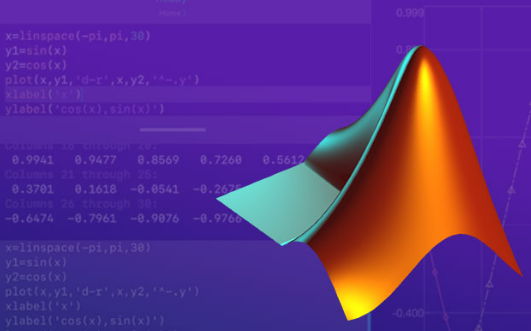
\includegraphics[width=0.7\columnwidth]{Figures/Figure0.png} %adding images
\end{figure}
%----------------------------------------------------------------------------------------
%	TABLE OF CONTENTS & LISTS OF FIGURES AND TABLES
%----------------------------------------------------------------------------------------

\makeatletter
\pretocmd{\chapter}{\addtocontents{toc}{\protect\addvspace{0\p@}}}{}{} %Controls spacing between table of contents
\pretocmd{\section}{\addtocontents{toc}{\protect\addvspace{7\p@}}}{}{}
\pretocmd{\subsection}{\addtocontents{toc}{\protect\addvspace{5\p@}}}{}{}
\makeatother

\setcounter{tocdepth}{2} %set the depth of the table of contents to show sections and subsections only 

\pagebreak
\tableofcontents % Print the table of contents
\listoffigures % Print the list of figures

%\listoftables % Print the list of tables

%----------------------------------------------------------------------------------------
%	Footnotes
%----------------------------------------------------------------------------------------

%\let\thefootnote\relax\footnotetext{\textsuperscript{1} \textit{Footnote 1 etc.}}

%\let\thefootnote\relax\footnotetext{\textsuperscript{2} \textit{Footnote 2 etc.}}

%----------------------------------------------------------------------------------------

\newpage % Start the article content on the second page, remove this if you have a longer abstract that goes onto the second page

%----------------------------------------------------------------------------------------
%	INTRODUCTION
%----------------------------------------------------------------------------------------

\section{MATLAB Basics\cite{MathWorks}}
%A statement requiring citation \cite{Figueredo:2009dg}.
\subsection{Data Types and Variables}
    \begin{enumerate}
	\item Data Types:
	\begin{itemize}
		\item Numeric Types: Integers (\texttt{int}), floating-point numbers (\texttt{float})
		
		Numeric types in MATLAB do not require explicit declaration of the type beforehand. You can assign values directly to variables, and the MATLAB interpreter will automatically recognize the appropriate numeric type based on the assigned value. Numeric types include integers (whole numbers) and floating-point numbers (decimal numbers).
		
		\textbf{Example:}
		\begin{verbatim}
			intNumber = 10;         % Integer
			floatNumber = 3.14;     % Floating-point number
		\end{verbatim}
		
		\item Characters: Single characters (\texttt{char})
		
		Characters in MATLAB are enclosed in single quotes (\texttt{'}). You can assign a single character to a variable. Characters are often used to represent individual symbols, letters, or digits.
		
		\textbf{Example:}
		\begin{verbatim}
			charValue = 'A';        % Character
		\end{verbatim}
		
		\item Strings: Sequence of characters (\texttt{string})
		
		Strings in MATLAB are enclosed in double quotes (\texttt{"}). You can assign a sequence of characters to a variable. Strings are commonly used to represent text or a collection of characters.
		
		\textbf{Example:}
		\begin{verbatim}
			stringValue = "Hello";  % String
		\end{verbatim}
		
		\item Logical: Boolean values (\texttt{true}, \texttt{false})
		
		Logical types in MATLAB represent boolean values, where \texttt{true} and \texttt{false} indicate the logical states. Logical values are used in conditional statements and logical operations.
		
		\textbf{Example:}
		\begin{verbatim}
			logicalValue = true;    % Logical value
		\end{verbatim}
	\end{itemize}
	
	\item Variables:
	\begin{itemize}
		\item Variable Declaration and Naming: Assigning values to variables
		
		In MATLAB, variables are assigned values using the assignment operator (\texttt{=}). The variable name is chosen by the programmer and can contain letters, numbers, and underscores. MATLAB is case-sensitive, so variable names in different cases are treated as different variables.
		
		\textbf{Example:}
		\begin{verbatim}
			variableName = value;
		\end{verbatim}
	\end{itemize}
\end{enumerate}

\subsection{Control Flow and Loops}
    \begin{enumerate}
	\item Control Flow:
	\begin{itemize}
		\item Conditional Statements: \texttt{if}, \texttt{else}, \texttt{elseif}
		
		Conditional statements allow you to control the flow of your program based on certain conditions. The \texttt{if} statement is used to execute a block of code if a condition is true. The \texttt{else} statement is optional and allows you to specify a block of code to execute if the condition is false. The \texttt{elseif} statement allows you to check additional conditions.
		
		\textbf{Example:}
		\begin{verbatim}
			if condition
			    statement;
			elseif condition
			    statement;
			else
			    statement;
			end
		\end{verbatim}
	\end{itemize}
	
	\item Loops:
	\begin{itemize}
		\item For Loop: Iterate a fixed number of times
		
		The \texttt{for} loop allows you to iterate a fixed number of times. You can specify the loop variable, the initial value, the increment, and the final value. The loop variable takes on each value in the specified range, and the statements inside the loop are executed for each iteration.
		\newline
		The \texttt{start:increment:end} operator is called the colon operator and it generates values from the start to the end with increments specified.
		
		\textbf{Example:}
		\begin{verbatim}
			for variable = start:increment:end
			    statement;
			end
		\end{verbatim}
		
		\item While Loop: Execute as long as a condition is true
		
		The \texttt{while} loop allows you to execute a block of code as long as a condition is true. The condition is checked at the beginning of each iteration. If the condition is true, the statements inside the loop are executed. The loop continues until the condition becomes false.
		
		\textbf{Example:}
		\begin{verbatim}
			while condition
			statement;
			end
		\end{verbatim}
	\end{itemize}
\end{enumerate}

\subsection{Functions and Modularity}
\begin{enumerate}
	\item Functions:
	\begin{itemize}
		\item Function Definition: Create reusable blocks of code
		
		Functions in MATLAB allow you to create modular and reusable blocks of code. A function is defined using the \texttt{function} keyword, followed by the function name, input arguments, and output arguments. The function body contains the statements to be executed, and the output values are assigned to the output arguments.
		
		\textbf{Example:}
		\begin{verbatim}
			function output = functionName(input)
			    statements;
			    output = value;
			end
		\end{verbatim}
		
		\item Function Call: Use the defined function
		
		To use a function, you can call it by its name and provide the necessary input arguments. The function will execute its code block and return the output values, which can be stored in variables for further use.
		
		\textbf{Example:}
		\begin{verbatim}
			result = functionName(input);
		\end{verbatim}
	\end{itemize}
	
	\item Built-in Math Functions:
	
	Math functions in MATLAB performs various mathematical operations on numeric data. These functions provide a wide range of capabilities for calculations involving absolute values, square roots, trigonometric operations, logarithms, and more.
	
	\textbf{Example:}
	\begin{verbatim}
		x = -5;
		abs_x = abs(x);             % Absolute value of x: 5
		
		y = 9;
		sqrt_y = sqrt(y);           % Square root of y: 3
		
		angle_deg = 45;
		angle_rad = deg2rad(angle_deg);     % Convert angle from degrees to radians
		
		sin_angle = sin(angle_rad);     % Sine of angle: 0.7071
		
		value = 1000;
		log_value = log10(value);   % Base-10 logarithm of value: 3
	\end{verbatim}
	
	The \texttt{abs()} function calculates the absolute value of \texttt{x}, the \texttt{sqrt()} function computes the square root of \texttt{y}, and the \texttt{log10()} function calculates the base-10 logarithm of \texttt{value}. The \texttt{deg2rad()} function is used to convert the \texttt{angle\_deg} variable from degrees to radians before computing the sine using the \texttt{sin()} function.
	
\end{enumerate}

\subsection{Arrays and Matrices}
\begin{enumerate}
	\item Arrays:
	\begin{itemize}
		\item Creating Arrays: Assigning values to arrays
		
		In MATLAB, arrays are used to store multiple values of the same type. You can create arrays using square brackets (\texttt{[ ]}) or by using built-in functions like \texttt{zeros}, \texttt{ones}, or \texttt{rand}.
		
		\textbf{Example:}
		\begin{verbatim}
			array = [1, 2, 3, 4, 5];           % Array with explicit values
			
			zerosArray = zeros(1, 5);          % Array of zeros
			onesArray = ones(1, 5);            % Array of ones
			randomArray = rand(1, 5);          % Array of random numbers
		\end{verbatim}
		
		\item Accessing Array Elements: Retrieving values from arrays
		
		You can access individual elements of an array using indexing. MATLAB uses one-based indexing, where the first element is at index 1.
		
		\textbf{Example:}
		\begin{verbatim}
			element = array(index);             % Accessing a specific element
		\end{verbatim}
	\end{itemize}
	
	\item Matrices:
	\begin{itemize}
		\item Creating Matrices: Assigning values to matrices
		
		Matrices are two-dimensional arrays that store multiple values in rows and columns. You can create matrices using square brackets (\texttt{[ ]}) or by using built-in functions like \texttt{zeros}, \texttt{ones}, or \texttt{rand}.
		
		\textbf{Example:}
		\begin{verbatim}
			matrix = [1, 2, 3; 4, 5, 6];             % Matrix with explicit values
			
			zerosMatrix = zeros(2, 3);               % Matrix of zeros
			onesMatrix = ones(2, 3);                 % Matrix of ones
			randomMatrix = rand(2, 3);               % Matrix of random numbers
		\end{verbatim}
		
		\item Accessing Matrix Elements: Retrieving values from matrices
		
		You can access individual elements of a matrix using indexing. The indexing format is \texttt{matrix(row, column)}. MATLAB uses one-based indexing.
		
		\textbf{Example:}
		\begin{verbatim}
			element = matrix(row, column);           % Accessing a specific element
		\end{verbatim}
	\end{itemize}
\end{enumerate}
\subsection{Console Input and Output}
\begin{enumerate}
	\item Input:
	\begin{itemize}
		\item Reading User Input: Prompting for user input
		
		You can use the \texttt{input} function to prompt the user for input during program execution. The user's input is captured as a string, and you can convert it to the appropriate data type if needed.
		
		\textbf{Example:}
		\begin{verbatim}
			userInput = input('Enter a value: ');       % Prompt for user input
		\end{verbatim}
	\end{itemize}
	
	\item Output:
	\begin{itemize}
		\item Displaying Output: Printing values to the console
		
		You can use the \texttt{disp} function to display output in the console. The function accepts multiple arguments and displays them as separate lines of output.
		
		\textbf{Example:}
		\begin{verbatim}
			disp('Hello, world!');                      % Display a message
			disp(variable);                             % Display a variable's value
		\end{verbatim}
	\end{itemize}
\end{enumerate}
\subsection{File Input and Output}
\begin{enumerate}
	\item Reading from Files:
	\begin{itemize}
		\item Reading Text Files: Loading text data from files
		
		You can use the \texttt{fread}, \texttt{fscanf}, or \texttt{readtable} functions to read data from text files. These functions allow you to read data in various formats, such as numeric values, strings, or tables.
		
		\textbf{Example:}
		\begin{verbatim}
			data = fread(fileID, size, precision);      % Read numeric data from a file
			data = fscanf(fileID, formatSpec);          % Read formatted data from a file
			data = readtable('data.txt');               % Read data into a table
		\end{verbatim}
	\end{itemize}
	
	\item Writing to Files:
	\begin{itemize}
		\item Writing Text Files: Saving data to text files
		
		You can use the \texttt{fwrite}, \texttt{fprintf}, or \texttt{writetable} functions to write data to text files. These functions allow you to write data in various formats, such as numeric values, strings, or tables.
		
		\textbf{Example:}
		\begin{verbatim}
			fwrite(fileID, data, precision);            % Write numeric data to a file
			fprintf(fileID, formatSpec, data);          % Write formatted data to a file
			writetable(data, 'output.txt');             % Write data from a table to a file
		\end{verbatim}
	\end{itemize}
\end{enumerate}
\subsection{Plotting and Visualization}
\begin{enumerate}
	\item Basic Plots:
	\begin{itemize}
		\item Line Plot: Plotting data as a line graph
		
		You can use the \texttt{plot} function to create line plots. The function accepts x and y values as input and generates a line graph based on the data.
		
		\textbf{Example:}
		\begin{verbatim}
			x = [1, 2, 3, 4, 5];
			y = [10, 15, 7, 9, 12];
			plot(x, y);
		\end{verbatim}
		
		\item Scatter Plot: Plotting data as individual points
		
		The \texttt{scatter} function allows you to create scatter plots. It takes x and y values as input and generates a plot with individual points representing the data.
		
		\textbf{Example:}
		\begin{verbatim}
			x = [1, 2, 3, 4, 5];
			y = [10, 15, 7, 9, 12];
			scatter(x, y);
		\end{verbatim}
	\end{itemize}
	
	\item Customizing Plots:
	\begin{itemize}
		\item Adding Labels and Titles: Providing information for the plot
		
		You can use functions like \texttt{xlabel}, \texttt{ylabel}, and \texttt{title} to add labels and titles to your plots. These functions allow you to provide additional information about the data being plotted.
		
		\textbf{Example:}
		\begin{verbatim}
			xlabel('X-axis');
			ylabel('Y-axis');
			title('Plot Title');
		\end{verbatim}
		
		\item Adding Legends: Differentiating multiple data series
		
		If you have multiple data series in a plot, you can use the \texttt{legend} function to add a legend that differentiates the series. The legend provides a visual representation of the data and helps identify each series.
		
		\textbf{Example:}
		\begin{verbatim}
			legend('Series 1', 'Series 2');
		\end{verbatim}
	\end{itemize}
\end{enumerate}

%----------------------------------------------------------------------------------------
%	CODE EXAMPLES
%----------------------------------------------------------------------------------------
\section{MATLAB Code Examples}
\subsection{Physics Programming Examples}

\begin{enumerate}
	\item \textbf{Calculating Projectile Motion}
	
	This example calculates the maximum height and range of a projectile launched at an angle, considering the effects of gravity. It utilizes variables, loops, conditions, and basic physics equations.
	
	\begin{verbatim}
		% Prompt the user for input
		v0 = input('Enter the initial velocity (m/s): ');
		theta = input('Enter the launch angle (degrees): ');
		g = 9.8;  % acceleration due to gravity (m/s^2)
		
		% Convert the angle from degrees to radians
		theta_rad = deg2rad(theta);
		
		% Calculate the time of flight
		t_flight = (2 * v0 * sin(theta_rad)) / g;
		
		% Calculate the maximum height
		h_max = (v0^2 * sin(theta_rad)^2) / (2 * g);
		
		% Calculate the horizontal range
		range = v0^2 * sin(2 * theta_rad) / g;
		
		% Display the results
		disp(['Time of flight: ', num2str(t_flight), ' seconds']);
		disp(['Maximum height: ', num2str(h_max), ' meters']);
		disp(['Horizontal range: ', num2str(range), ' meters']);
	\end{verbatim}
	
	This program prompts the user to enter the initial velocity (\texttt{v0}) and launch angle (\texttt{theta}) of a projectile. It then calculates the time of flight, maximum height, and horizontal range using the provided inputs and the equations of projectile motion. The calculated values are displayed using the \texttt{disp} function.
	
	\item \textbf{Calculating Electric Field Intensity}
	
	This example calculates the electric field intensity at a point due to a point charge. It uses variables, conditions, and basic physics equations related to Coulomb's law.
	
	\begin{verbatim}
		% Prompt the user for input
		k = 9e9;  % Coulomb's constant (Nm^2/C^2)
		q = input('Enter the charge (C): ');
		r = input('Enter the distance from the charge (m): ');
		
		% Calculate the electric field intensity
		E = k * abs(q) / r^2;
		
		% Display the result
		disp(['Electric Field Intensity: ', num2str(E), ' N/C']);
	\end{verbatim}
	
	This program prompts the user to enter the charge (\texttt{q}) and distance (\texttt{r}) from the charge to the point where the electric field intensity is to be calculated. It then applies Coulomb's law equation to calculate the electric field intensity (\texttt{E}). The calculated value is displayed using the \texttt{disp} function.
	
\end{enumerate}

\subsection{MATLAB Plotting Example}

\begin{enumerate}
	\setcounter{enumi}{2}
	
	\item \textbf{Plotting a Sine Function}
	
	This example demonstrates how to plot a sine function using MATLAB's plotting capabilities.
	
	\begin{verbatim}
		% Generate x values from 0 to 2*pi
		x = 0:0.01:2*pi;
		
		% Calculate y values as the sine of x
		y = sin(x);
		
		% Plot the sine function
		plot(x, y);
		
		% Add labels and title
		xlabel('x');
		ylabel('sin(x)');
		title('Plot of the Sine Function');
	\end{verbatim}
	
	This program generates a set of x-values ranging from 0 to $2\pi$ using the colon operator (\texttt{0:0.01:2*pi}). It then calculates the corresponding y-values as the sine of the x-values (\texttt{y = sin(x)}). Finally, it plots the sine function by calling the \texttt{plot} function with the x and y values as arguments. The \texttt{xlabel}, \texttt{ylabel}, and \texttt{title} functions are used to add labels and a title to the plot. The output is shown in Fig. 1
	
\end{enumerate}


\begin{figure}[H]
\centering %A statement requiring citation \cite{Figueredo:2009dg}
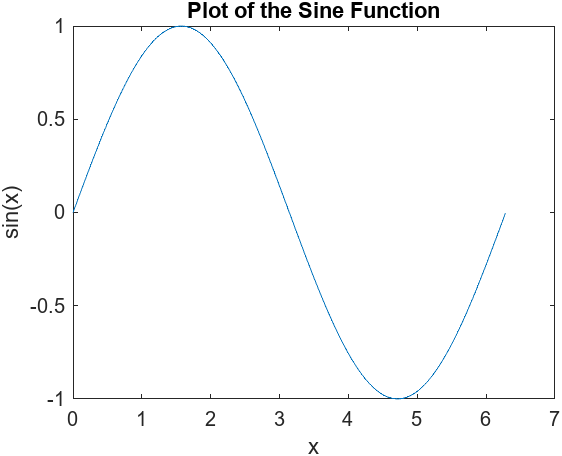
\includegraphics[width=0.4\columnwidth]{Figures/Figure1.png} 
\caption[Sine Function Plot]{Sine Function Plot} % The text in the square bracket is the caption for the list of figures while the text in the curly brackets is the figure caption
\label{fig:gallery} 
\end{figure}

%----------------------------------------------------------------------------------------
%	BIBLIOGRAPHY
%----------------------------------------------------------------------------------------
\renewcommand{\refname}{\spacedlowsmallcaps{References}} % For modifying the bibliography heading
\raggedright
\bibliographystyle{unsrt}

\bibliography{sample.bib} % The file containing the bibliography

%----------------------------------------------------------------------------------------

\end{document}